%%%%%%%%%%%%%%%%%%%%%% 
%%Options for presentations (in-class) and handouts (e.g. print). 
\documentclass[pdf]{beamer} 
%\documentclass[pdf,handout]{beamer}
%\usepackage{pgfpages}
%\pgfpagesuselayout{2 on 1}[letterpaper,border shrink=5mm]

%%%%%%%%%%%%%%%%%%%%%%
%Change this for different slides so it appears in bar
\usepackage{authoraftertitle}
\date{$\mathbb{R}^n$: Vectors}

\graphicspath{{../}}

%%%%%%%%%%%%%%%%%%%%%%
%% Upload common style file
\usepackage{../LyryxLinearAlgebraSlidesStyle}



\begin{document}
	
	%%%%%%%%%%%%%%%%%%%%%%%
	%% Title Page and Copyright Common to All Slides	
	%Title Page
	\input ../frontmatter/titlepage.tex	
	%LOTS Page
	%\input frontmatter/lyryxopentexts.tex	
	%Copyright Page
	\input ../frontmatter/copyright.tex	
	%%%%%%%%%%%%%%%%%%%%%%%%%


{\small
\section{What is Rn?}
%--------------------startslide-----------------------------%
\frame{\frametitle{What is $\RR^n$?}
\begin{block}{Notation and Terminology}
%\pause
\begin{itemize}
\item \alert{$\RR$} denotes the set of \alert{real numbers}.
%\pause
\item \alert{$\RR^2$} denotes the set of
all \alert{column vectors with two entries}.
%\pause
\item \alert{$\RR^3$} denotes the set of
all \alert{column vectors with three entries}.
%\pause
\item In general, \alert{$\RR^n$} denotes the
set of all \alert{column vectors with $n$ entries}.
\end{itemize}
\end{block}
}
%-------------- end slide -------------------------------%

%-------------- start slide -------------------------------%
\frame{\frametitle{Scalar quantities versus vector quantities}
\begin{block}{}
\begin{itemize}
\item
A \alert{scalar} quantity has only magnitude;
e.g.\ time, temperature.
%\pause
\item
A (non-zero) \alert{vector} quantity has both magnitude and direction;
e.g.\ displacement, force, wind velocity.
\end{itemize}
\pause
Whereas two scalar quantities are equal if they are represented
by the same value, 
two vector quantities are equal if and only if they have
the same \alert{magnitude} and \alert{direction}.
\end{block}
}
%-------------- end slide -------------------------------%


%-------------- start slide -------------------------------%
\frame{
\begin{alertblock}{$\RR^2$ and $\RR^3$}
Vectors in $\RR^2$ and $\RR^3$ have convenient geometric
representations as {\bf position vectors} of points in
the 2-dimensional (Cartesian) plane and in 3-dimensional
space, respectively.
\end{alertblock}
}
%-------------- end slide -------------------------------%

%-------------- start slide -------------------------------%
\frame{
\begin{picture}(4,2.5)
\put(0.3,0.7){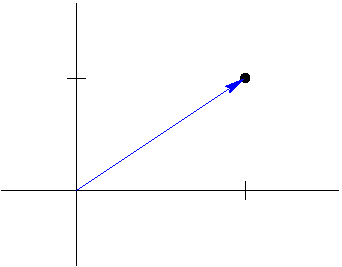
\includegraphics[scale=0.7]{figures/R2.pdf}}
\put(0.2,2.2){{$\RR^2$}}
\put(0.5,0.9){\scriptsize{$0$}}
\put(1.7,0.95){\scriptsize{$x$}}
\put(1.4,0.9){\scriptsize{$a$}}
\put(0.55,1.9){\scriptsize{$y$}}
\put(0.5,1.55){\scriptsize{$b$}}
\put(1.5,1.6){\scriptsize{\alert{$(a,b)$}}}
%\pause
\put(0.5,0.3){\scriptsize\textcolor{blue}{The vector
$\left[\begin{array}{c} a \\ b\end{array}\right]$.}}
%\pause
\put(2.4,2.4){{$\RR^3$}}
\put(2.5,0.3){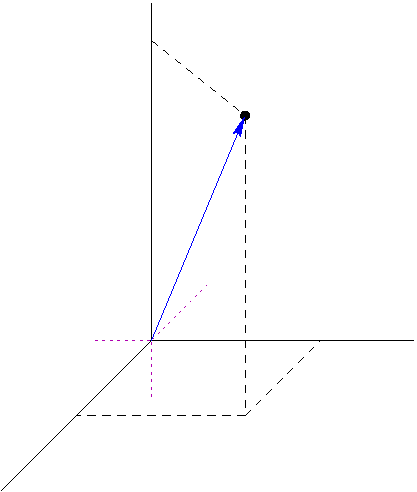
\includegraphics[scale=0.7]{figures/R3.pdf}}
\put(3.05,1.1){\scriptsize{$0$}}
\put(2.45,0.4){\scriptsize{$x$}}
\put(4.3,0.9){\scriptsize{$y$}}
\put(3.18,2.65){\scriptsize{$z$}}
\put(3.75,2.05){\scriptsize{\alert{$(a,b,c)$}}}
\put(2.7,0.65){\scriptsize{$a$}}
\put(3.95,1.05){\scriptsize{$b$}}
\put(3.05,2.45){\scriptsize{$c$}}
%\pause
\put(3.0,0.1){\scriptsize\textcolor{blue}{The vector
$\left[\begin{array}{c} a \\ b \\c \end{array}\right]$.}}
\end{picture}
}
%-------------- end slide -------------------------------%

%-----------------------start slide-----------------------%
\frame{
\begin{block}{Notation}
\begin{itemize}
\item If $P$ is a point in $\mathbb{R}^n$ with coordinates $(p_1, p_2, ...,p_n)$ we denote this by $P = (p_1, p_2, ..., p_n)$. 
\pause
\item
If $P=(p_1, p_2, \ldots, p_n)$ is a point in $\RR^n$, then 
\[\longvect{0P}=\left[\begin{array}{c}
p_1 \\ p_2 \\ \vdots \\ p_n \end{array}\right] \]
is often used to
denote the position vector of the point.
\pause
\item
Instead of using a capital letter to denote the vector
(as we generally do with matrices), we emphasize the 
importance of the geometry and the direction with
an arrow over the name of the vector. 

\end{itemize}
\end{block}
}
%-------------- end slide -------------------------------%


%-------------- start slide -------------------------------%
\frame{
\begin{block}{Notation and Terminology}
\begin{itemize}
\item
The notation $\longvect{0P}$ emphasizes that this vector goes from the origin $0$ to the point $P$. We can also use lower case letters for names of vectors. In this case, we write $\longvect{0P} = \vect{p}$. 
\pause
\item Any vector
\[ \vect{x} =\left[\begin{array}{c} x_1 \\ x_2 \\ \vdots \\ x_n\end{array}\right]
\mbox{ in } \RR^n \]
is associated with the 
\alert{point $(x_1, x_2, \ldots, x_n)$}.
%\pause
\item Often,
\alert{there is no distinction made between the vector $\vect{x}$ and the
point $(x_1, x_2, \ldots, x_n)$}, %\pause 
and we say that both
\alert{$(x_1, x_2, \ldots, x_n) \in \RR^n$ and $\vect{x} =\left[\begin{array}{c} x_1 \\ x_2 \\ \vdots \\ x_n\end{array}\right] \in \mathbb{R}^n$.}
\end{itemize}
\end{block}

}
%-------------- end slide -------------------------------%

\section{Geometric Vectors}
%-------------- start slide -------------------------------%
\frame{\frametitle{Geometric Vectors in $\RR^2$ and $\RR^3$}
\begin{block}{}
Let $A$ and $B$ be two points in $\RR^2$ or $\RR^3$.
%\pause
\begin{picture}(3,2.2)
\put(0.1,0){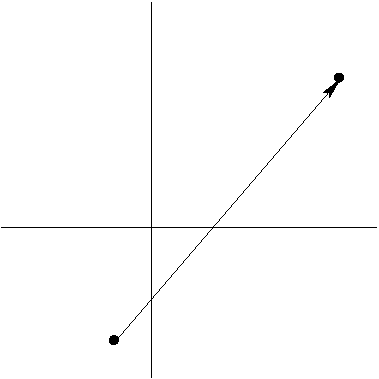
\includegraphics[scale=.75]{figures/vectors-1.pdf}}
\put(0.75,0.65){\small $0$}
\put(1.8,0.65){\small $x$}
\put(0.75,1.7){\small $y$}
\put(1.65,1.5){\small $B$}
\put(0.5,0.15){\small $A$}
\pause
\put(2.2,1.5){\small $\bullet$ $\longvect{AB}$ is the
\alert{geometric vector} from $A$ to $B$.}
\pause
\put(2.2,1.3){\small $\bullet$ $A$ is the \alert{tail} of
$\longvect{AB}$.}
%\pause
\put(2.2,1.1){\small $\bullet$ $B$ is the \alert{tip} of
$\longvect{AB}$.}
%\pause
\put(2.2,0.9){\small $\bullet$ the \alert{magnitude} of
$\longvect{AB}$ is its length, and is}
\put(2.32,0.72){\small denoted $||\longvect{AB}||$.}
\end{picture}
\end{block}
}
%-------------- end slide -------------------------------%

%-------------- start slide -------------------------------%
\frame{
\begin{block}{Equality of geometric vectors}
\begin{picture}(3,2.2)
\put(0.1,0){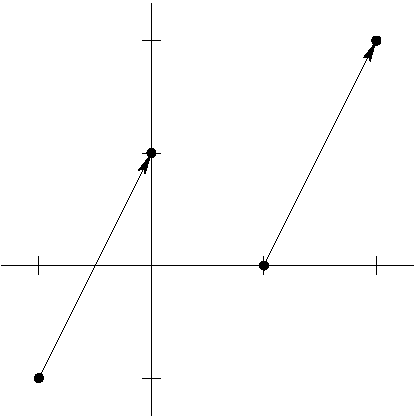
\includegraphics[scale=.75]{figures/vectors-2.pdf}}
\put(0.75,0.65){\small $0$}
\put(2.1,0.65){\small $x$}
\put(0.75,2.0){\small $y$}
\put(1.3,0.60){\small $A$}
\put(1.8,1.85){\small $B$}
\put(0.15,0.15){\small $C$}
\put(0.7,1.3){\small $D$}
\pause
\put(2.3,1.6){\small $\bullet$ $\longvect{AB}$ is the
vector from $A=(1,0)$.}
\put(2.43,1.4){\small to $B=(2,2)$.}
%\pause
\put(2.3,1.2){\small $\bullet$ $\longvect{CD}$ is the
vector from $C=(-1,-1)$}
\put(2.43,1.0){\small to $D=(0,1)$.}
\pause
\put(2.3,0.5){\small $\bullet$
$\longvect{AB} = \longvect{CD}$ 
because the vectors have}
\put(2.43,0.35){\small the same \alert{length}
and \alert{direction}.}
\end{picture}
\pause

The fact that the points $A$ and $B$ are different from the
points $C$ and $D$ is not important.
%\pause 
For geometric vectors,
\alert{the location of the vector in the plane (or in 3-dimensional
space) is not important};
%\pause
the important properties are its length and direction.
\end{block}
}
%-------------- end slide -------------------------------%

%-------------- start slide -------------------------------%
\frame{
\begin{block}{Coordinatizing Vectors -- Part 1}

\begin{picture}(3,1.8)
\put(0.4,0){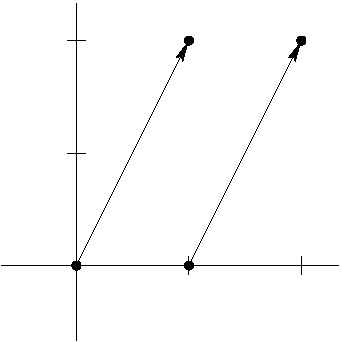
\includegraphics[scale=.75]{figures/vectors-3.pdf}}
\put(0.65,0.25){\footnotesize $0$}
\put(2.0,0.25){\footnotesize $x$}
\put(0.65,1.6){\footnotesize $y$}
\put(1.25,0.2){\footnotesize $A$}
\put(1.95,1.45){\footnotesize $B$}
\put(1.2,1.45){\footnotesize $P$}
%\pause
\put(2.4,1){$\longvect{0P}$ is the \alert{position vector} for
$P=(1,2)$,}
%\pause
\put(2.4,0.7){and $\longvect{0P}
=\left[\begin{array}{c}
1 \\ 2 \end{array}\right]$.}
\end{picture}
\bigskip
\pause

Since $\longvect{AB}=\longvect{0P}$,
%\pause
\alert{it should be the case that 
$\longvect{AB}= \left[\begin{array}{c}
1 \\ 2 \end{array}\right]$}.
%\pause
This can be seen by moving $\longvect{AB}$ so that its
tail is at the origin.
\end{block}
\pause
\begin{alertblock}{}
A geometric vector is coordinatized by putting
it in \alert{standard position},
meaning with its tail at the origin,
and then identifying the vector with its tip.
\end{alertblock}
}
%-------------- end slide -------------------------------%

\section{Algebra in Rn}
%--------------------start slide---------------------------%
\frame{\frametitle{Algebra in $\RR^n$}
%\pause
\begin{block}{Addition in $\RR^n$}
Since vectors in $\RR^n$ are $n\times 1$ matrices, addition in $\RR^n$ is precisely matrix
addition using column matrices,
%\pause
i.e., 
\begin{itemize}
\item If $\vect{u}$ and $\vect{v}$ are in $\RR^n$, then 
$\vect{u}+\vect{v}$ is obtained by adding together corresponding 
entries of the vectors.
%\pause
\item
The zero vector in $\RR^n$ is the $n\times 1$ zero matrix, and
is denoted $\vect{0}$.
\end{itemize}
\end{block}

\pause

\begin{example}
Let $\vect{u} = \left[
\begin{array}{r}
1 \\
2 \\
3 
\end{array}
\right]$ and $\vect{v} = \left[
\begin{array}{r}
4 \\
5 \\
6 
\end{array}
\right]$. Then, 
\[
\vect{u} + \vect{v}  = \left[
\begin{array}{r}
1 \\
2 \\
3 
\end{array}
\right] + \left[
\begin{array}{r}
4 \\
5 \\
6 
\end{array}
\right]
=
\left[
\begin{array}{r}
5 \\
7 \\
9 
\end{array}
\right]
\]
\end{example}
}
%-------------- end slide -------------------------------%

%------------------start slide--------------------%
\frame{\frametitle{Properties of Vector Addition}

\begin{block}{}
Let $\vect{u}, \vect{v},$ and $\vect{w}$ be vectors in $\mathbb{R}^n$.
Then the following properties hold.
\pause
\begin{enumerate}
\item
$\vect{u} + \vect{v} = \vect{v} + \vect{u}$
\hfill\textcolor{blue}{(vector addition is commutative)}.
\pause
\item
$(\vect{u} + \vect{v}) + \vect{w} = \vect{u} + (\vect{v} + \vect{w})$
\hfill\textcolor{blue}{(vector addition is associative)}.
\pause
\item
$\vect{u} + \vect{0} = \vect{u}$
\hfill\textcolor{blue}{(existence of an additive identity)}.
\pause
\item
$\vect{u} + (-\vect{u}) = \vect{0}$
\hfill\textcolor{blue}{(existence of an additive inverse)}.
\end{enumerate}
\end{block}
}
%--------------------end slide-------------------%

%--------------------start slide---------------%
\frame{\frametitle{Scalar Multiplication}

\begin{block}{}
Since vectors in $\RR^n$ are $n\times 1$ matrices, scalar multiplication in $\RR^n$ is precisely matrix
scalar multiplication using column matrices,
%\pause
i.e., 
If $\vect{u}$ is a vector in $\RR^n$ and $k\in\RR$ is a
scalar, then $k\vect{u}$ is obtained by multiplying every
entry of $\vect{u}$ by $k$.
\end{block}

\pause

\begin{example}
Let $\vect{u} = \left[
\begin{array}{r}
1 \\
2 \\
3 
\end{array}
\right]$ and $k = 4$. 
Then, 
\[
k\vect{u} = 4 \left[
\begin{array}{r}
1 \\
2 \\
3 
\end{array}
\right] = \left[
\begin{array}{r}
4 \\
8 \\
12 
\end{array}
\right]
\]
\end{example}
}

%--------------------end slide------------------------%

%--------------------start slide---------------------------%
\frame{\frametitle{Properties of Scalar Multiplication}

\begin{block}{}
Let $\vect{u}, \vect{v} \in \mathbb{R}^n$ be vectors
and $k, p\in \RR$ be scalars.
Then  the following properties hold.
\pause
\begin{enumerate}
\item
$k (\vect{u} + \vect{v}) = k\vect{u} + k\vect{v}$
\hfill\textcolor{blue}{(scalar multiplication distributes over
vector addition)}.
\pause
\item
$(k + p) \vect{u} = k\vect{u} + p\vect{u}$
\hfill\textcolor{blue}{(addition distributes over
scalar multiplication)}.
\pause
\item
$k(p\vect{u}) = (kp)\vect{u}$
\hfill\textcolor{blue}{(scalar multiplication is associative)}.
\pause
\item
$1\vect{u} = \vect{u}$
\hfill\textcolor{blue}{(existence of a multiplicative identity)}.
\end{enumerate}
\end{block}
}
%-------------- end slide -------------------------------%
%-------------- start slide -------------------------------%
\frame{\frametitle{Some notation you may encounter }

\begin{block}{}
Often, in $ \mathbb{R}^2 $ the notation $ \displaystyle \vec{i} = 
\left[\begin{array}{c}
1 \\  0 \end{array}\right],
\vec{j} = 
\left[\begin{array}{c}
0 \\ 1  \end{array}\right] $ is used. Whereas in $ \mathbb{R}^3 $ the notation is
$\displaystyle \vec{i} = 
\left[\begin{array}{c}
1 \\ 0 \\ 0 \end{array}\right],
\vec{j} = 
\left[\begin{array}{c}
0 \\ 1 \\ 0 \end{array}\right],\vec{k} = 
\left[\begin{array}{c}
0 \\ 0 \\ 1 \end{array}\right] $

So we have  
\[
\left[\begin{array}{c}
a \\  b \end{array}\right] = a\vec{i}+b\vec{j}
\]

and 
\[\left[\begin{array}{c}
a \\ b \\ c \end{array}\right] = a\vec{i}+b\vec{j}+c\vec{k}
\]
\end{block}
}
%-------------- end slide -------------------------------%

\section{The Geometry of Vector Addition}
%--------------------start slide---------------------------%
\frame{\frametitle{The Geometry of Vector Addition}
%\pause
\begin{block}{}
\begin{enumerate}
\item
\alert{Vector Equality.} The vectors have the same length and direction.
\pause
\item
\alert{The zero vector, $\vec{0}$} has length zero and
\alert{no direction}.
\pause
\item
\alert{Addition}. 
Let $\vec{u},\vec{v}$ be vectors. 
Then $\vec{u}+\vec{v}$ is the diagonal of
the \alert{parallelogram defined by $\vec{u}$ and $\vec{v}$},
and having the same tail as $\vec{u}$ and $\vec{v}$.
\end{enumerate}
%\pause
\begin{picture}(3.5,1.0)
\put(1.4,0){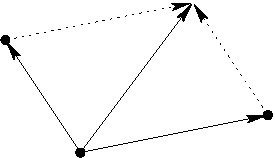
\includegraphics[scale=0.9]{figures/vectors-4.pdf}}
\put(1.5,0.3){$\vec{u}$}
\put(1.95,0.6){$\vec{u}+\vec{v}$}
\put(2.6,0.0){$\vec{v}$}
\end{picture}
\bigskip

\end{block}
}
%-------------- end slide -------------------------------%

%-------------- start slide -------------------------------%
\frame{
\begin{block}{Tip-to-Tail Method for Vector Addition}
For points $A$, $B$ and $C$,
\[ \longvect{AB} + \longvect{BC}
=\longvect{AC}.\]
\bigskip

\begin{picture}(3.5,1.2)
\put(1.4,0){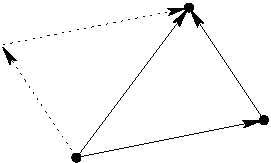
\includegraphics[scale=1]{figures/vectors-5.pdf}}
\put(1.8,-0.1){\small $A$}
\put(3.25,0.25){\small $B$}
\put(2.65,1.15){\small $C$}
\put(2.5,-0.1){\small$\longvect{AB}$}
\put(3.0,0.6){\small$\longvect{BC}$}
\put(2.05,0.6){\small$\longvect{AC}$}
\put(1.9,1.0){\tiny$\longvect{AB}$}
\put(1.5,0.25){\tiny$\longvect{BC}$}
\end{picture}
\vspace*{.2in}

\end{block}
}
%-------------- end slide -------------------------------%

%-------------- start slide -------------------------------%
\frame{
\begin{example}
The diagonals of any parallelogram bisect each other.
\pause
\medskip

To see this,
denote the parallelogram by its vertices, $ABCD$.

\begin{picture}(2.5,1.3)
\put(0.2,0.2){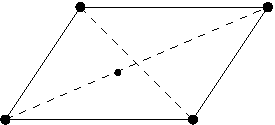
\includegraphics[scale=1]{figures/vectors-6.pdf}}
\put(0.1,0.1){\small{$A$}}
\put(0.55,1){\small{$B$}}
\put(2.05,1){\small{$C$}}
\put(1.5,0.1){\small{$D$}}
\put(0.9,0.6){\tiny{$M$}}
\pause
\put(2.5,.9){$\bullet$ Let $M$ denote the midpoint}
\put(2.65,.7){of $\longvect{AC}$.}
\pause
\put(2.65,.5){Then $\longvect{AM}=\longvect{MC}$.}
\pause
\put(2.5,.3){$\bullet$ It now suffices to show}
\put(2.65,.1){that $\longvect{BM}=\longvect{MD}$.}
\end{picture}
\pause

\[ \longvect{BM}
\pause
= \longvect{BA} +\longvect{AM} 
\pause
= \longvect{CD} +\longvect{MC} 
\pause
= \longvect{MC} +\longvect{CD} 
\pause
= \longvect{MD}.\]
\pause
Since $\longvect{BM}=\longvect{MD}$, these
vectors have the same \alert{magnitude} and 
\alert{direction},
\pause
implying that $M$ is the midpoint of $\longvect{BD}$.
\pause
\medskip

Therefore, the diagonals of $ABCD$ bisect each other.
\end{example}
}
%-------------- end slide -------------------------------%

%-------------- start slide -------------------------------%
\frame{
\begin{block}{The Geometry of Vector Subtraction}
Let $\vec{u}$ and $\vec{v}$ be vectors in $\RR^2$ or $\RR^3$.
%\pause
The vector $\alert{\vec{u}-\vec{v}} = \vec{u} + (-\vec{v})$
is obtained from the parallelogram defined by $\vec{u}$ and $\vec{v}$
%\pause
by taking the vector from the tip of $\vec{v}$ to the
tip of $\vec{u}$,
%\pause 
i.e., the diagonal of the parallelogram,
directed towards the tip of $\vec{u}$.
%\pause

\begin{picture}(2.5,1.0)
\put(1.2,0){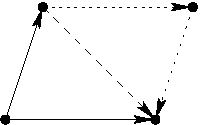
\includegraphics[scale=1]{figures/vectors-7.pdf}}
\put(1.2,0.4){\small{$\vec{v}$}}
\put(1.65,-0.1){\small{$\vec{u}$}}
\put(1.9,0.85){\small{$\vec{u}$}}
\put(2.4,0.4){\small{$-\vec{v}$}}
\put(1.9,0.4){\small{$\vec{u}-\vec{v}$}}
\end{picture}
\bigskip

\end{block}
}
%------------------end slide----------------------------%

%--------------------start slide---------------------------%
\frame{
\begin{block}{Coordinatizing Vectors -- Part 2}
Let $A=(x_1, y_1, z_1)$ and $B=(x_2,y_2,z_2)$ be two points in
$\RR^3$.  
%\pause 

\begin{picture}(2.5,1.5)
\put(1.4,0){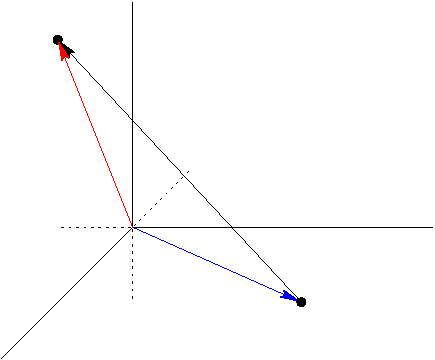
\includegraphics[scale=0.6]{figures/vectors-distance.pdf}}
\put(1.9,0.4){\scriptsize{$0$}}
\put(1.4,0.1){\scriptsize{$x$}}
\put(3,0.4){\scriptsize{$y$}}
\put(2.0,1.3){\scriptsize{$z$}}
\put(2.68,0.2){\scriptsize{\textcolor{blue}{$A$}}}
\put(1.45,1.3){\scriptsize{\alert{$B$}}}
\end{picture}
\pause

We see from the figure that
$\longvect{0A} + \longvect{AB}=\longvect{0B}$,
and hence
%\pause
\[
\longvect{AB} = \longvect{0B}-\longvect{0A} 
%\pause
= 
\left[\begin{array}{c} x_2 \\ y_2 \\ z_2 \end{array}\right] 
-
\left[\begin{array}{c} x_1 \\ y_1 \\ z_1 \end{array}\right] 
%\pause
=
\left[\begin{array}{c} x_2 -x_1 \\ y_2 -y_1 \\ z_2 -z_1 \end{array}\right].
\]
\end{block}
}
%------------------end slide----------------------------%

\section{Length of a Vector}
%--------------------start slide---------------------------%
\frame{\frametitle{Length of a Vector, $\mathbb{R}^2$}

If $\vect{x}=\left[\begin{array}{c} x_1 \\ x_2\end{array}\right] 
\in\RR^2$, 

\begin{picture}(3,0.7)
\put(1.5,0){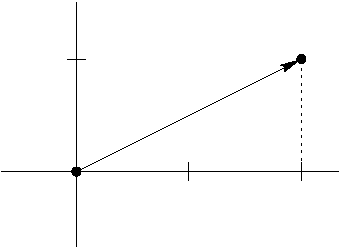
\includegraphics[scale=.6]{figures/vectors-length.pdf}}
\put(1.7,0.18){\footnotesize $0$}
\put(2.9,0.27){\footnotesize $x$}
\put(1.7,0.9){\footnotesize $y$}
\put(2.8,0.75){\footnotesize $X = (x_1,x_2)$}
\put(2.2,0.6){\footnotesize $\vect{x}$}
\end{picture}
%\pause

then the length of the vector $\vect{x}$ is the distance from the origin $0$ to the point $X = (x_1, x_2)$ given by $d(0,X)$. 

%\pause
\begin{block}{}
The length of $\vect{x}$, denoted $\vectlength \vect{x} \vectlength$, is given by:
\[ d(0,X) = \vectlength \vect{x} \vectlength =\sqrt{x_1^2 + x_2^2}.\]
\end{block}
}
%----------------end slide---------------------%

%------------start slide------------------%
\frame{\frametitle{Length of a Vector, $\mathbb{R}^3$}

This extends clearly to $\vect{x}=\left[\begin{array}{c} x_1 \\ x_2 \\ x_3 \end{array}\right] \in\RR^3$.

%\pause

The length of $\vect{x}$ is the distance from the origin $0$ to the point $X = (x_1, x_2, x_3)$ given by $d(0,X)$. 

%\pause

\begin{block}{}
\[ d(0,X) = \vectlength \vect{x} \vectlength =\sqrt{x_1^2 + x_2^2 + x_3^2}.\]
\end{block}

\pause

\begin{alertblock}{}
Suppose we want to find the distance between points other than the origin?
\end{alertblock}
}
%-------------------end slide-------------------%

%---------------start slide------------------------%
\frame{\frametitle{Length of a Vector, $\mathbb{R}^3$}

Consider two arbitrary points in $\mathbb{R}^3$, $A=(x_1, y_1, z_1)$ and $B=(x_2,y_2,z_2)$. Then the distance between them is written $d(A,B)$ and is given by the \alert{distance formula}.

\begin{block}{Distance Formula}
\[ d(A,B) =
\sqrt{(x_2-x_1)^2 + (y_2-y_1)^2 +(z_2-z_1)^2} .  \]
\end{block}
\smallskip

\pause
Now let $P = (x_2-x_1, y_2-y_1, z_2-z_1)$, and 
\[
\vect{p} = \left[ \begin{array}{c}
x_2-x_1 \\
y_2-y_1 \\
z_2-z_1
\end{array}
\right]
\]

\pause
Then the length of $\vect{p}$ is equal to the distance between the origin and $P$, which are both equal to the distance between points $A$ and $B$
\pause
\begin{block}{}
\[ \vectlength \vect{p} \vectlength = d(0,P)= d(A,B) =
\sqrt{(x_2-x_1)^2 + (y_2-y_1)^2 +(z_2-z_1)^2} .  \]
\end{block}

}
%-------------- end slide -------------------------------%

%--------------------start slide---------------------------%
\frame{\frametitle{Length of a Vector, $\mathbb{R}^n$}

\begin{block}{}
More generally, if $P=(p_1, p_2, \ldots, p_n)$ and
$Q=(q_1, q_2, \ldots, q_n)$ are points in $\RR^n$, then
\alert{the distance between $P$ and $Q$} is the length of
the vector $\longvect{PQ}$, written $\vectlength \longvect{PQ} \vectlength$. 
\[ d(P,Q) = \vectlength \longvect{PQ} \vectlength =
\sqrt{(q_1-p_1)^2 +(q_2-p_2)^2 + \cdots +(q_n-p_n)^2}.\]
\end{block}
\pause

\begin{block}{}
The formula for calculating the length of a vector
generalizes to $\RR^n$:
%\pause 
if \[ \vect{x}=\left[\begin{array}{c} x_1 \\ x_2 \\ \vdots \\ x_n 
\end{array}\right] \in\RR^n,\]
%\pause
then
\[ \vectlength \vect{x} \vectlength =\sqrt{x_1^2 + x_2^2 + \cdots + x_n^2},\]
%\pause
which represents the distance from the origin to the point
$(x_1, x_2, \ldots, x_n)$.
\end{block}
}
%-------------- end slide -------------------------------%

%----------------------start slide--------------------%
\frame{\frametitle{Properties of Distance}

\begin{block}{}
Let $P$ and $Q$ be two points in $\mathbb{R}^n$,
and $d(P,Q)$ the distance between them.
%\pause
Then the following properties hold.
\pause
\begin{enumerate}
\item
The distance between $P$ and $Q$ is equal to the distance
between $Q$ and $P$,
%\pause
i.e., $d(P,Q)=d(Q,P)$.
\pause
\item
$d(P,Q)\geq 0$ with equality if and only if $P=Q$.
\end{enumerate}
\end{block}

\pause

\begin{example}
For $P=(1,-1,3)$ and $Q=(3,1,0)$, the distance between $P$ and $Q$ is
$d(P,Q)= \sqrt{2^2 + 2^2 + (-3)^2}
=\sqrt{17}$.
\end{example}

}
%-------------------end slide-----------------%

%-------------- start slide -------------------------------%
\frame{
\begin{example}
Let $\vec{p}=
\left[\begin{array}{c}
-3 \\ 4 \end{array}\right]$ and
$\vec{q}=
\left[\begin{array}{c}
3 \\ -1 \\ -2 \end{array}\right]$.
Then
$-2\vec{q}=(-2)\vec{q}=
\left[\begin{array}{c}
-6 \\ 2 \\ 4 \end{array}\right]$.
\pause

The lengths of these vectors are
\[ \vectlength \vec{p} \vectlength  = \sqrt{(-3)^2 + 4^2} =\sqrt{9+16} = 5,\]
\pause
\[ \vectlength \vec{q} \vectlength  = \sqrt{(3)^2 + (-1)^2 + (-2)^2}
=\sqrt{9+1 + 4} = \sqrt{14},\]
\pause
and
\begin{eqnarray*}
\vectlength -2\vec{q} \vectlength & = & \sqrt{(-6)^2 + 2^2 + 4^2} \\
& = & \sqrt{36+4 + 16}\\
& = & \sqrt{56} = \sqrt{4\times 14}\\
& = & 2\sqrt{14} = 2 \vectlength\vec{q} \vectlength.
\end{eqnarray*}
\end{example}
}
%-------------- end slide -------------------------------%

\section{The Geometry of Scalar Multiplication}

%--------------------start slide-------------------------%
\frame{\frametitle{The Geometry of Scalar Multiplication}

\begin{block}{}
\begin{itemize}
\item
\alert{Scalar Multiplication.}
If $\vec{v}\neq\vec{0}$ and $a\in\RR$, $a\neq 0$,
then $a\vec{v}$ has length 
$\vectlength a\vect{v}\vectlength=|a|\cdot \vectlength\vec{v}\vectlength$, and
\pause
\begin{itemize}
\item has the same direction as $\vec{v}$ if $a>0$;
\pause
\item has direction opposite to $\vec{v}$ if $a<0$.
\end{itemize}
\pause
\item
\alert{Parallel Vectors.}
Two nonzero vectors are called \alert{parallel} if 
they have the same direction or opposite directions.
\pause
It follows that nonzero vectors \alert{$\vec{v}$ and $\vec{w}$ are parallel
if and only if one is a scalar multiple of the other.}
\end{itemize}
\end{block}
}
%------------------------end slide----------------------%


%--------------------start slide---------------------------%
\frame{
\begin{problem}\em
Let $P=(1,-2,1)$,$Q=(-3,0,5)$, $X=(2, -1, 5)$ and $Y=(4,-2,3)$
be points in $\RR^3$.
Is $\longvect{PQ}$ parallel to $\longvect{XY}$?
Is $\longvect{PX}$ parallel to $\longvect{QY}$?
\end{problem}
\pause
\begin{solution}\em
$\longvect{PQ} =
\left[\begin{array}{r} -4 \\ 2 \\ 4 \end{array}\right]$,
\pause
$\longvect{XY} =
\left[\begin{array}{r} 2 \\ -1 \\ -2 \end{array}\right]$,
\pause
and these vectors are parallel if
$\longvect{PQ} = k\longvect{XY}$ for some 
scalar $k$, 
\pause
i.e.,
\vspace*{-.1in}

\[
\left[\begin{array}{r} -4 \\ 2 \\ 4 \end{array}\right]
=k\left[\begin{array}{r} 2 \\ -1 \\ -2 \end{array}\right]
\pause
\mbox{ or }
\left[\begin{array}{r} -4 \\ 2 \\ 4 \end{array}\right]
=\left[\begin{array}{r} 2k \\ -k \\ -2k \end{array}\right].
\]
\vspace*{-.1in}

\pause
This gives a system of three equations in one variable,
\pause
which is consistent, and has unique solution $k=-2$.
\pause
\alert{Therefore, $\longvect{PQ}$ 
is parallel to $\longvect{XY}$.}
\pause
\medskip

$\longvect{PX} =
\left[\begin{array}{r} 1 \\ 1 \\ 4 \end{array}\right]$,
\pause
$\longvect{QY} =
\left[\begin{array}{r} 7 \\ -2 \\ -2 \end{array}\right]$,
\pause
and these vectors are parallel if
$\longvect{PX} = \ell\longvect{QY}$ for some 
scalar $\ell$.
\pause
\alert{You will find that no such $\ell$ exists, so
$\longvect{PX}$ 
is not parallel to $\longvect{QY}$.}

\end{solution}
}
%-------------- end slide -------------------------------%

\section{Unit Vectors}

%--------------------start slide---------------------------%
\frame{\frametitle{Unit Vectors}
\begin{definition}
A \alert{unit vector} is a vector of length one.
\end{definition}
\pause
\begin{example}
$\left[\begin{array}{c}
1 \\ 0 \\ 0
\end{array}\right]$, 
$\left[\begin{array}{c}
0 \\ 1 \\ 0
\end{array}\right]$, 
$\left[\begin{array}{c}
0 \\ 0 \\ 1
\end{array}\right]$, 
$\left[\begin{array}{c}
\frac{\sqrt{2}}{2} \\ 0 \\ \frac{\sqrt{2}}{2}
\end{array}\right]$, 
are examples of unit vectors.
\end{example}
\pause

\begin{example}
If $\vec{v}\neq\vec{0}$, then 
\[ \frac{1}{ \vectlength \vec{v} \vectlength} \vec{v} \]
is a unit vector in the same direction as $\vec{v}$.
\end{example}
}
%-------------- end slide -------------------------------%

%--------------------start slide---------------------------%
\frame{
\begin{example}
$\vec{v}=\left[\begin{array}{r}
-1 \\ 3 \\ 2
\end{array}\right]$
is not a unit vector, since $\vectlength \vec{v} \vectlength =\sqrt{14}$.
\pause
However,
\vspace*{-.2in}

\[ \vec{u}=\frac{1}{\sqrt{14}}\vec{v}
=\left[\begin{array}{c}\vspace*{.02in}
\frac{-1}{\sqrt{14}} \\ \vspace*{.02in}
\frac{3}{\sqrt{14}} \\
\frac{2}{\sqrt{14}} \end{array}\right]\]
\vspace*{-.1in}

is a unit vector \alert{in the same direction} as $\vec{v}$,
\pause
i.e.,
\[ \vectlength \vec{u} \vectlength =
\frac{1}{\sqrt{14}} \vectlength \vec{v} \vectlength 
=\frac{1}{\sqrt{14}} \sqrt{14}=1.\]
\end{example}
\pause
\begin{example}
If $\vec{v}$ and $\vec{w}$ are nonzero that have
\begin{itemize}
\item
the same direction, then
$\vec{v}=\frac{\vectlength \vec{v} \vectlength }{\vectlength \vec{w} \vectlength}\vec{w}$;
\pause
\item
opposite directions, then
$\vec{v}=-\frac{\vectlength \vec{v} \vectlength }{\vectlength \vec{w} \vectlength }\vec{w}$.
\end{itemize}
\end{example}
}
%-------------- end slide -------------------------------%




\section{Vector problems and examples}
%-------------- start slide -------------------------------%
\frame{\frametitle{Vector problems and examples}
\begin{problem}\em
Find the point, $M$, that is midway between $P_1=(-1,-4,3)$
and $P_2=(5,0,-3)$.
\end{problem}
\pause
\begin{solution}\em
\begin{picture}(2.5,0.9)
\put(1.5,0.1){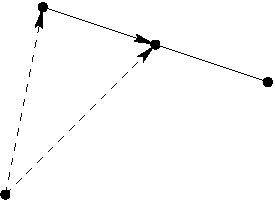
\includegraphics[scale=.6]{figures/vectors-9.pdf}}
\put(1.45,0){\scriptsize $0$}
\put(1.45,0.85){\scriptsize $P_1$}
\put(2.1,0.78){\scriptsize $M$}
\put(2.65,0.5){\scriptsize $P_2$}
\end{picture}
\pause
\vspace*{-.3in}

\begin{eqnarray*}
\longvect{0M}
\pause
= \longvect{0P_1}
+ \longvect{P_1M}
\pause
=\longvect{0P_1}
+\frac{1}{2} \longvect{P_1P_2}
\pause
& = &
\left[\begin{array}{r}
-1 \\ -4 \\ 3
\end{array}\right]
+ \frac{1}{2}
\left[\begin{array}{r}
6 \\ 4 \\ -6
\end{array}\right] \\
\pause
& = &
\left[\begin{array}{r}
-1 \\ -4 \\ 3
\end{array}\right]
+
\left[\begin{array}{r}
3 \\ 2 \\ -3
\end{array}\right]
\pause
=
\left[\begin{array}{r}
2 \\ -2 \\ 0
\end{array}\right].
\end{eqnarray*} 
\pause
Therefore $M=(2,-2,0)$.
\end{solution}
}
%-------------- end slide -------------------------------%

%-------------- start slide -------------------------------%
\frame{
\begin{problem}\em
Find the two points trisecting the segment between $P=(2,3,5)$
and $Q=(8,-6,2)$.
\end{problem}
\pause
\begin{solution}\em
\begin{picture}(2.5,0.9)
\put(0.5,0.1){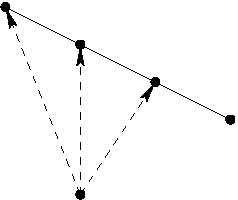
\includegraphics[scale=.6]{figures/vectors-10.pdf}}
\put(0.75,0){\scriptsize $0$}
\put(0.35,0.85){\scriptsize $P$}
\put(0.8,0.8){\scriptsize $A$}
\put(1.1,0.65){\scriptsize $B$}
\put(1.5,0.4){\scriptsize $Q$}
\pause
\put(2.2,0.75){\footnotesize{$\bullet$ $\longvect{0A}
= \longvect{0P} + \frac{1}{3} \longvect{PQ}$}}
\pause
\put(2.2,0.5){\footnotesize{$\bullet$ $\longvect{0B}
= \longvect{0P} + \frac{2}{3} \longvect{PQ}$}}
\end{picture}
\pause

Since $\longvect{PQ}=
\left[\begin{array}{r}
6 \\ -9 \\ -3
\end{array}\right]$,
\pause
\[ \longvect{0A}=
\left[\begin{array}{r}
2 \\ 3 \\ 5
\end{array}\right]
+
\left[\begin{array}{r}
2 \\ -3 \\ -1
\end{array}\right]
=\left[\begin{array}{r}
4 \\ 0 \\ 4
\end{array}\right]
\pause \mbox{ and }~
\longvect{0B}=
\left[\begin{array}{r}
2 \\ 3 \\ 5
\end{array}\right]
+
\left[\begin{array}{r}
4 \\ -6 \\ -2
\end{array}\right]
=\left[\begin{array}{r}
6 \\ -3 \\ 3
\end{array}\right].\]  
\pause
Therefore, the two points are $A=(4,0,4)$ and $B=(6,-3,3)$.
\end{solution}
}
%-------------- end slide -------------------------------%

%-------------- start slide -------------------------------%
\frame{
\begin{example}
If $ABCD$ is an arbitrary quadrilateral, then the
the midpoints of the four sides of $ABCD$ are the
vertices of a parallelogram.
\pause

\begin{picture}(2.5,1.4)
\put(0.2,0.1){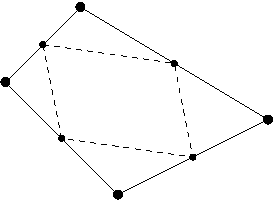
\includegraphics[scale=0.9]{figures/vectors-11.pdf}}
\put(0.05,0.75){\small $A$}
\put(0.5,1.2){\small $B$}
\put(1.85,0.55){\small $C$}
\put(0.7,0){\small $D$}
\pause
\put(2.2,1.1){\small Let $M_1$ denote the
midpoint of $\longvect{AB}$,}
\put(0.3,1.05){\tiny $M_1$}
\pause
\put(2.43,0.9){\small $M_2$ the midpoint of $\longvect{BC}$,}
\put(1.25,1.0){\tiny $M_2$}
\pause
\put(2.43,0.7){\small $M_3$ the midpoint of $\longvect{CD}$, and}
\put(1.35,0.25){\tiny $M_3$}
\pause
\put(2.43,0.5){\small $M_4$ the midpoint of $\longvect{DA}$.}
\put(0.4,0.35){\tiny $M_4$}
\end{picture}
\pause

It suffices to prove that
$\longvect{M_1M_2} = \longvect{M_4M_3}$.
\pause

\[\begin{array}{rclcrcl}
\longvect{M_1M_2}
& = & \longvect{M_1B} +\longvect{BM_2} 
& \hspace*{.4in}\uncover<11->{ 
\longvect{M_4M_3}
& = & \longvect{M_4D} +\longvect{DM_3} } \\
\pause
& = & \frac{1}{2}\longvect{AB} +\frac{1}{2}\longvect{BC} 
& \uncover<12->{ 
& = & \frac{1}{2}\longvect{AD} +\frac{1}{2}\longvect{DC} } \\
\pause
& = & \frac{1}{2}\longvect{AC}
& \uncover<13->{ 
& = & \frac{1}{2}\longvect{AC}}
\end{array}\]
\uncover<14->{
Since $\longvect{M_1M_2} = \longvect{M_4M_3}$,
the points $M_1$, $M_2$, $M_3$, $M_4$ are the vertices of
a parallelogram.}
\end{example}
}
%-------------- end slide -------------------------------%

}\end{document}

%--------------------start slide---------------------------%
%-------------- end slide -------------------------------%

%--------------------start slide---------------------------%
%----------------------end slide---------------------------%

%-------------- start slide -------------------------------%
%-------------- end slide -------------------------------%

%-------------- start slide -------------------------------%
%-------------- end slide -------------------------------%

%--------------------start slide--------------------------%

%----------------------start slide------------------%
%-------------------end slide----------------------------%

%-------------- start slide -------------------------------%
%-------------- end slide -------------------------------%

%-------------- start slide -------------------------------%
%-------------------end slide--------------------%

%----------------------start slide---------------%
%-------------- end slide -------------------------------%
